\documentclass[journal]{IEEEtran}

\usepackage{xeCJK} % CJK语言环境,使用XeLaTex进行编译
\usepackage{authblk} % 对应中文部分的作者机构特殊语法

% 将 authblk 包中的作者连词 and 替换为中文逗号
\renewcommand*{\Authsep}{,}
\renewcommand*{\Authand}{,}
\renewcommand*{\Authands}{,}

\setlength{\parindent}{2em} %2em代表首行缩进两个字符

%行间距
\usepackage{setspace} % 用于设置行间距

\onehalfspacing%设置1.5倍行距
%字号
\fontsize{22pt}{\baselineskip}{\selectfont}

%设置英文正文字体
\setmainfont{Times New Roman}
\usepackage{fontspec}

%图片
\usepackage{graphicx} %插入图片的宏包
\usepackage{float} %设置图片浮动位置的宏包
\usepackage{subfigure} %插入多图时用子图显示的宏包

\usepackage[justification=centering]{caption}

%段间距
\setlength{\parskip}{1pt}

% 设置图注编号为图1-1格式
\captionsetup[figure]{labelformat=simple, labelsep=quad, font={small, singlespacing}, justification=raggedright}

\captionsetup[table]{labelformat=simple, labelsep=quad, font={small, singlespacing}, justification=raggedright}

\renewcommand{\thefigure}{\arabic{section}-\arabic{figure}}

%引用
\usepackage{cite}

% correct bad hyphenation here
\hyphenation{op-tical net-works semi-conduc-tor}

\begin{document}

% paper title
\title{基于YOLOv8的头盔检测模型\\设计与实现}

\author{陈邵杰,郭昊,蔡明珠,刘政,黄俊毅,王晶昊,杨双菁,田睿朴,苗馨月% <-this % stops a space
\thanks{感谢电子科技大学机器学习课程闫老师与张老师的教学。}% <-this % stops a space
\thanks{2024年10月}}


% The paper headers
\markboth{Journal of \LaTeX\ Class Files,~Vol.~14, No.~8, October~2015}%
{Shell \MakeLowercase{\textit{et al.}}: 机器学习课程设计报告}


% make the title area
\maketitle

% As a general rule, do not put math, special symbols or citations
% in the abstract or keywords.
\begin{abstract}
随着人工智能的发展和交通安全需求的增加,基于深度学习的目标检测技术在行人头盔佩戴检测中发挥着重要用。在本研究中,针对行人检测场景采用YOLOv8l模型进行头盔检测,并通过稀疏化和剪枝技术对模型进行优化,在高精度的同时提升推理效率。利用稀疏化方法对YOLOv8l模型的权重进行优化,增强模型的稀疏性,减少计算冗余。通过剪枝技术有效去除冗余的网络参数和连接,大幅减少模型的计算量和参数规模,优化后的模型在嵌入式和边缘计算设备上运行效率显著提升。实验结果表明,经过稀疏化和剪枝后的YOLOv8l模型参数量减少了约30\%,推理速度提高了近40\%,并且在行人头盔检测任务中维持了高达98\%的准确率。我们还将优化后的模型与YOLOv3、YOLOv5、YOLOv7等多个版本进行了对比,验证了YOLOv8l在行人检测精度和速度方面的优势。
\end{abstract}

% Note that keywords are not normally used for peerreview papers.
\begin{IEEEkeywords}
交通管理,YOLOv8,头盔检测,深度学习,目标检测
\end{IEEEkeywords}

\IEEEpeerreviewmaketitle

%1 引言
\section{引言}

%1.1课题背景及意义
\subsection{选题背景与意义}
Subsection text here.
%1.1.1课题背景
\subsubsection{课题背景}
subsubsection text here.
%1.1.1研究意义
\subsubsection{研究意义}
subsubsection text here.

%1.2研究问题分析
\subsection{研究问题分析}
Subsection text here.

%2 引言
\section{行人数据图像处理}
The conclusion goes here.

%2.1 实验数据集
\subsection{实验数据集}
Subsection text here.A'
%2.2 图像预处理
\subsection{图像预处理}
Subsection text here.
%2.3 yolo标准数据集
\subsection{yolo标准数据集}
Subsection text here.
%2.4 数据集标注
\subsection{数据集标注}
Subsection text here.

%3 基于YOLOv8的检测系统实现
\section{基于YOLOv8的检测系统实现}
YOLOv8是一种精准高效的目标检测解决方案,系统采用YOLOv8作为核心检测算法,识别电动车及其驾驶员,并判断是否存在佩戴头盔行为。训练与测试使用的均为540*355的YOLO标准数据集,图3-1为整个实验流程图:
\begin{figure}[htbp] 

   \centering
   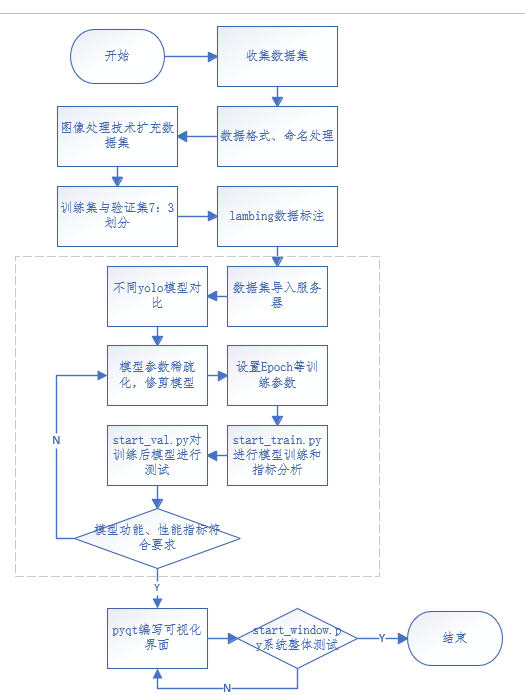
\includegraphics[width=8cm]{figures/流程图.png}
   \caption{实验流程图} 
   \label{fig:} 
  
\end{figure} 

%3.1 训练环境搭建
\subsection{训练环境搭建}
对于大量图片数据集与复杂模型,通过GPU进行模型训练大加速,通过AutoDL平台租借云服务器实现YOLOv8模型的搭建,训练,测试与部署工作。\par
本次实验使用的硬件环境为:CPU 16 vCPU Intel(R) Xeon(R) Platinum 8481C,GPU RTX 4090D,显存大小24G,硬盘为80G。\par
软件环境:操作系统ubutnu22.04,编程语言python版本3.8.5,pytorch版本1.10.0,Cuda版本11.8。\par

%3.2 模型训练
\subsection{模型训练}
本次实验采用YOLOv8模型进行目标检测训练,整个训练过程依托于高性能服务器硬件及成熟的软件环境,确保了模型的高效收敛和稳定性能。\par
训练流程从数据准备开始,输入图像维度为像素540*355,首先对数据集进行了精细的标注、清洗和划分,形成训练集、验证集和测试集,为模型的训练和评估提供了坚实的数据基础。并且通过高性能硬件配置使得数据处理与模型计算可以高效并行执行,显著提高了训练效率。\par
整个训练过程共进行了100个epoch,训练阶段首先加载数据集,并进行数据增强操作,提高模型的泛化能力。接着初始化YOLOv8模型,设置包括学习率和批次大小等超参数,以确保训练初期能够有效学习特征。每个epoch包含前向传播、损失计算、反向传播和权重更新等步骤。\par
在服务器上,GPU的强大算力极大加速了这些运算,在卷积层的特征提取和参数更新过程中尤为显著。每个epoch结束后,模型会在验证集上进行评估,以监控性能并避免过拟合的发生。训练日志详细记录了每个epoch的损失、精度和召回率等关键指标,并且实时生成了损失曲线和精度曲线,以便于监控训练过程中的动态表现和分析模型的改进方向。\par
在进行模型参数配置时,为了确保对比实验的一致性和准确性,我们需要核心参数固定不变,以排除对训练效果产生的潜在影响。训练epoch为100轮,使用随机梯度下降优化器,初始学习率和周期学习率均设置为0.01,设置batch数量为64。经训练,YOLOv8模型最终达到了预期的检测效果,能够精准地识别目标物体,表现出良好的鲁棒性和检测性能。通过数据预处理、模型初始化、迭代训练和模型评估的完整闭环与高性能服务器硬件的支持,使得模型在合理时间内完成了高效训练。\par

%3.3 模型部署
\subsection{模型部署}
\begin{figure}[htbp] 

   \centering
   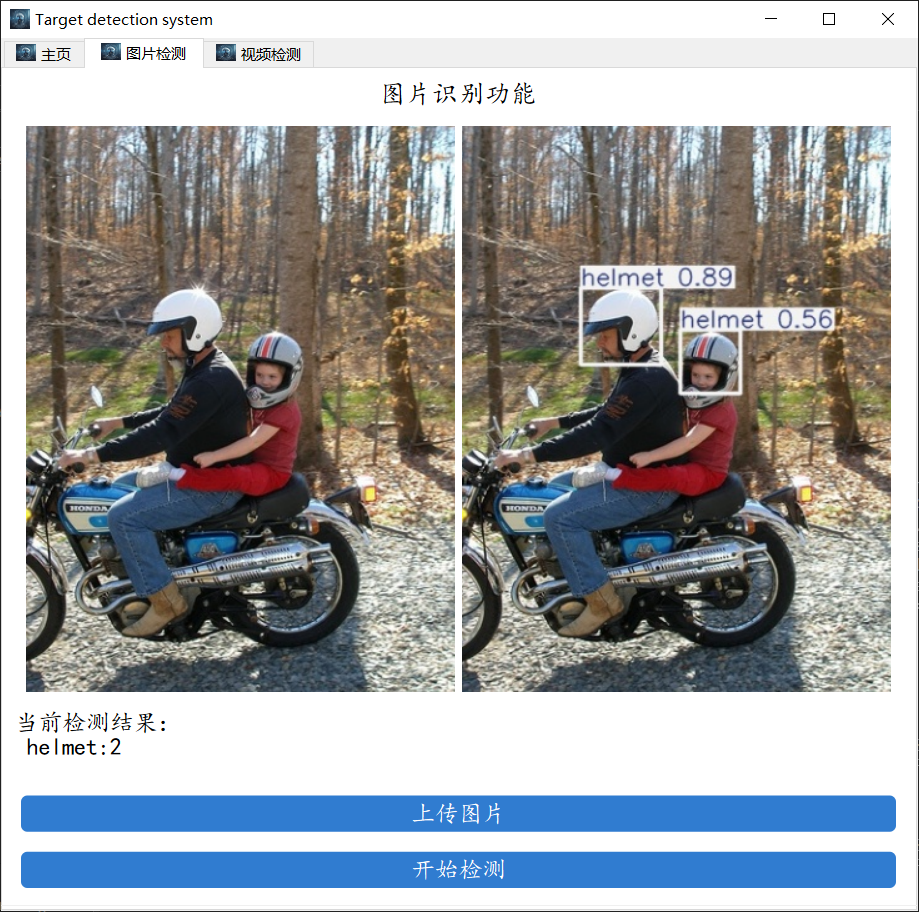
\includegraphics[width=8cm]{figures/部署页面.png}
   \caption{部署界面} 
   \label{fig:} 
  
\end{figure} 

%4 调整与改进
\section{调整与改进}
电动自行车头盔的检测可能由于骑手的高速移动或环境的复杂性而变得颇具挑战性。例如,头盔可能因与摄像头距离较远而成为难以辨识的小目标。针对检测过程中低分辨率图像及小目标检测困难,背景与检测目标相似等问题,改进Yolov8n 模型。传统目标检测网络容易忽略或误判电动车骑行过程中远处、边缘或比例较小的头盔,进而导致漏检或误检。对此需要增强原始YOLOv8n模型以提升对小目标检测精度。\par

%4.1 卷积注意力模块
\subsection{卷积注意力模块}
本研究模型加入了基于卷积注意力机制模块\textsuperscript{\cite{1}}(Convolutional Block Attention Module, CBAM)的小目标检测优化策略。CBAM作为一种即插即用的注意力机制模块,可直接嵌入至多种流行的卷积神经网络架构中。该模块通过对输入特征图的不同区域赋予不同的权重,使网络能够更加聚焦于对特定任务具有重要性的信息,同时忽略不相关的信息。因此,在针对佩戴头盔的行人检测任务中,由于目标与摄像头距离较远导致行人及头盔尺寸较小,且在检测图像中所占比例较低,引入CBAM能够使网络更加专注于前景中的小目标,并有效定位感兴趣的区域。这进一步增强了网络的特征提取能力,使得在最小感受野的特征图上能够更精确地识别小目标。CBAM的总体架构如图4-1所示。\par
\begin{figure}[htbp] 

   \centering
   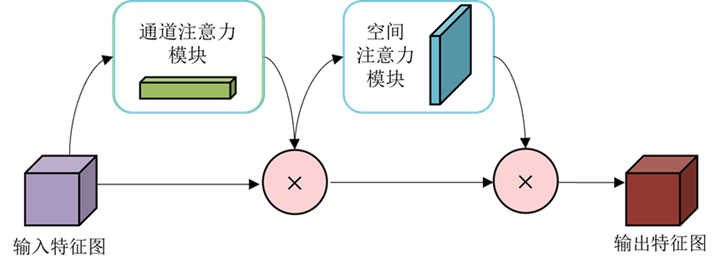
\includegraphics[width=8cm]{figures/4_1.png}
   \caption{CBAM结构图} 
   \label{fig:} 
  
\end{figure} 
对于输入特征图 ,CBAM先使用通道注意力模块,在宽高维度上对输入进行平均池化和最大池化的操作,得到两个 大小的张量。然后,将两个张量分别经过共享卷积层,将输出进行逐元素相加,再经过非线性激活操作,得到通道注意力权值,即大小为 的张量。将该权值与输入特征图进行逐元素相乘,得到通道注意力模块的输出特征图 。接着,对于通道注意力模块的输出特征图,在通道维度上进行平均池化和最大池化操作,得到两个 大小的张量。然后,将两个张量在通道维度上进行拼接,并经过一个卷积操作,将通道维度降为1。最终,经过非线性激活操作,得到空间注意力权值,即大小为 的张量。将该权值与通道注意力模块的输出特征图进行逐元素相乘,便得到经过卷积注意力模块处理后的输出特征图。根据论文[1]中的实验结果,在不同的图像分类和目标检测数据集上,将CBAM集成到不同的神经网络模型中后,模型的性能得到很大的提高,这证明了该模块的有效性。\par
针对YOLOv8n网络,本文将卷积注意力CBAM模块应用在了特征金字塔网络下采样过程中的每一个跨阶段局部模块之后,对不同层次的特征进行融合的Neck部分,模型框架修改后如2所示。\par
\begin{figure}[htbp] 

   \centering
   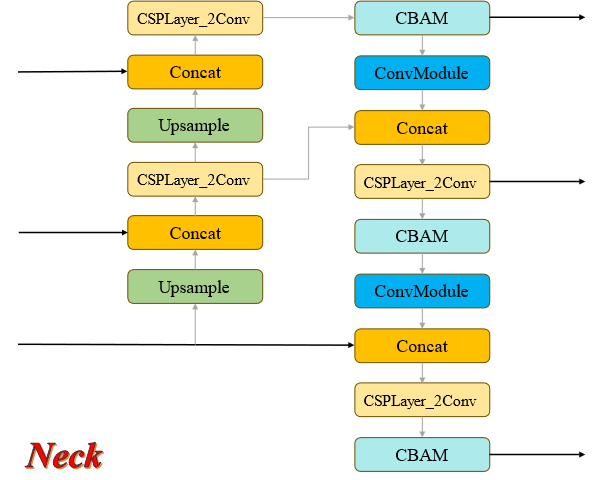
\includegraphics[width=8cm]{figures/4_2.png}
   \caption{应用CBAM卷积注意力模块网络Neck部分结构图} 
   \label{fig:} 
  
\end{figure} 
%4.2 Transformer Block
\subsection{Transformer Block}
Transformer\textsuperscript{\cite{2}}是一种专为处理序列数据而设计的深度学习架构。该模型利用自注意力机制实现了高效的并行计算,并具备捕获长距离依赖关系的能力。\par
Transformer的结构如图3所示,主要由编码器和解码器两大部分构成。编码器负责将输入信息映射为中间的隐藏状态表示,而解码器则将这些隐藏状态转换为最终的输出序列。编码器由若干相同的编码器层堆叠而成,每一层均包含自注意力机制和前馈神经网络。解码器在结构上与编码器相似,但额外增加了一个注意力层,该层用于关注编码器的输出。\par
多头自注意力机制是Transformer的核心,它使得模型在处理输入序列时能够同时关注序列中不同位置的信息。查询、键和值通过不同的线性变换分成多组(头),然后对每组进行自注意力计算,最后将所有头的输出拼接起来,再次通过一个线性层得到最终的输出。\par
前馈网络是注意力机制之后的一个关键组件。对注意力层的输出进行进一步的非线性变换,以捕获更复杂的特征和表示。\par
\begin{figure}[htbp] 

   \centering
   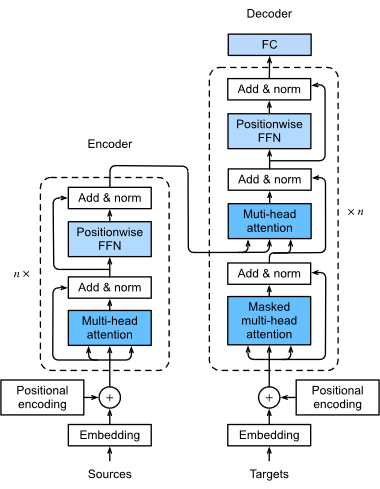
\includegraphics[width=8cm]{figures/4_3.png}
   \caption{Transformer结构图} 
   \label{fig:} 
  
\end{figure} 
针对YOLOv8n网络,本文在特征处理的中间层C2f中加入Transformer模块,修改后的C2f结构如图4所示。通过引入自注意力机制,修改后的模型能够更好地捕捉长距离依赖关系,这有助于模型在处理图像时能够更好地理解全局上下文信息,从而提升特征的表示能力。且由于Transformer block能够有效捕捉全局信息,从而帮助模型在不同的尺度上捕捉到小目标的特征,能够更好地区分头盔与复杂的背景。此外,在YOLOv8n的架构中,特征融合是一个关键环节。Transformer block可以作为一种有效的特征融合工具,通过自注意力机制融合不同层次的特征信息,提高模型在各种环境下的鲁棒性,减少误报和漏报,进一步提升检测性能。\par
\begin{figure}[htbp] 

   \centering
   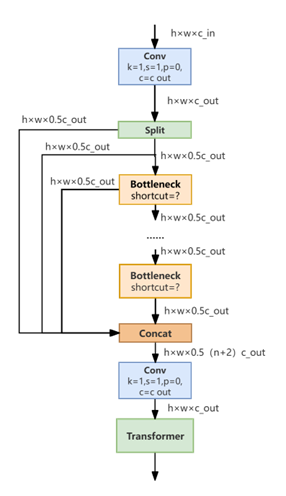
\includegraphics[width=8cm]{figures/4_4.png}
   \caption{添加Transformer后的C2f结构图} 
   \label{fig:} 
  
\end{figure} 
%4.3 
\subsection{创新点3}
Subsection text here.

%5 实验结果
\section{实验结果}
The conclusion goes here.

%6 总结与展望
\section{总结与展望}
The conclusion goes here.

% if have a single appendix:
%\appendix[Proof of the Zonklar Equations]
% or
%\appendix  % for no appendix heading
% do not use \section anymore after \appendix, only \section*
% is possibly needed

% use appendices with more than one appendix
% then use \section to start each appendix
% you must declare a \section before using any
% \subsection or using \label (\appendices by itself
% starts a section numbered zero.)
%

% use section* for acknowledgment
\section*{致谢}


The authors would like to thank...


% Can use something like this to put references on a page
% by themselves when using endfloat and the captionsoff option.
\ifCLASSOPTIONcaptionsoff
  \newpage
\fi



% 参考文献
\begin{thebibliography}{1}

\bibitem{1}
Woo S, Park J, Lee J Y, et al. CBAM: Convolutional block attention module[C]//Proceedings of the European conference on computer vision (ECCV). 2018: 3-19.

\bibitem{2}
Vaswani A. Attention is all you need[J]. Advances in Neural Information Processing Systems, 2017.

\end{thebibliography}


% that's all folks
\end{document}


